\section{Algorithms Used}\label{section:algorithms-used}
To count the number of occurrences of every word in a book, an exact counter and two different probabilistic counters were used.
The two different probabilist counters were a fixed probability counter and a Csűrös' counter.

\subsection{Exact Counter Algorithm}
An exact counter is a data structure that maintains an accurate count of unique items in a stream of data.
In this specific case, the counter maintains an accurate count of words inside a book. 

In this algorithm, an empty data structure is created.
This data structure creates a subdivision for every new word accounted for.
Inside that subdivision, an integer keeps count of every account of that specific word.
This can be better visualised in \autoref{alg:exact}.

\begin{algorithm}
\caption{Exact counter algorithm}
\label{alg:exact}
\begin{algorithmic}
\Inputs{$book \gets$ string of text to be analysed}
\Initialize{$counter \gets$ data structure used for counting the occurrences of every word}

\For{$word$ in $book$}

    \If{$word$ in $counter$}
        \State $counter[word]+=1$
    \Else
        \State $counter[word] \gets$ data structure
    \EndIf
\EndFor
\end{algorithmic}
\end{algorithm}


% This algorithm was developed by resourcing to the \verb|Counter| data structure from the library \verb|collections| in Python
This algorithm allows for an exact count of unique items, with no error margin. 
The downside of using an exact counter is that it can use a lot of memory.

\subsection{Fixed probabilistic counter}
A fixed probabilistic counter is a data structure that keeps count of the number of distinct elements in a stream of data, with a certain level of precision. 
It employs random sampling to determine the count and the degree of accuracy can be altered by altering the probability of sampling.
This probabilty remains constant for the entire duration of the algorithm.

Similarly to \autoref{alg:exact}, an empty data structure is created.
Every time a new word is analysed, a random number from 0 to 1 is generated.
If this number is lower than the sampling probability, then the word is sampled.
If a subdivision for the sampled word does not exist inside the data structure, this division is created.
Inside that subdivision, an integer keeps count of every account of that specific sampled word.
This algorithm is explained in \autoref{alg:fixed}.

% \clearpage

\begin{algorithm}[ht!]
\caption{Fixed probability counter algorithm}
\label{alg:fixed}
\begin{algorithmic}
\Inputs{$book \gets$ string of text to be analysed

$p \gets$ sampling probability }
\Initialize{$counter \gets$ data structure used for counting the occurrences of every word
            $RandomNumber \gets$ function that generates a number between 0 and 1}



\For{$word$ in $book$}
    $r_{number} = RandomNumber$
    \If{$r_{number}<p$}

        \If{$word$ in $counter$}
            \State $counter[word]+=1$
        \Else
            \State $counter[word] \gets$ data structure
            \State $counter[word]=1$
        \EndIf

    \EndIf
\EndFor
\end{algorithmic}
\end{algorithm}

For a specific number of occurrences $x$ with $p$ being the sampling probability, to calculate the expected count $f(x)$, it is used:

\begin{equation}
    f(x) = \frac{x}{p}
    \label{eq:fixed}
\end{equation}


\subsection{Csűrös' probabilty counter algorithm}
Another type of probabilistic counter are the counters with decreasing probabilty.
A decreasing probabilistic counter is, similarly to a fixed probabilistic counter, a data structure that keeps count of the number of distinct elements in a stream of data, with a certain level of precision. 
It also employs random sampling to determine the count.
However, the sampling probabilty decreases as the algorithm evolves.
This allows for an accurate count in the first occurrences of an event without using to much memory.

One example of this type of counter is the Csűrös' counter. %TODO add citation
This is a floating-point counter defined with the aid of a design parameter $M = 2^d$, where d is a nonnegative integer.
This counter counts with deterministic updates for the first $M$ occurrence, similarly to \autoref{alg:exact}.
The next updates are probabilistic, with the next $M$ updates having a probability of $\frac{1}{2}$, followed by $M$ updates with probabilty of $\frac{1}{4}$, etc...
This algorithm is described in \autoref{fig:csuros} and \autoref{alg:csuros}.

\begin{figure}[!ht]
    \centering
    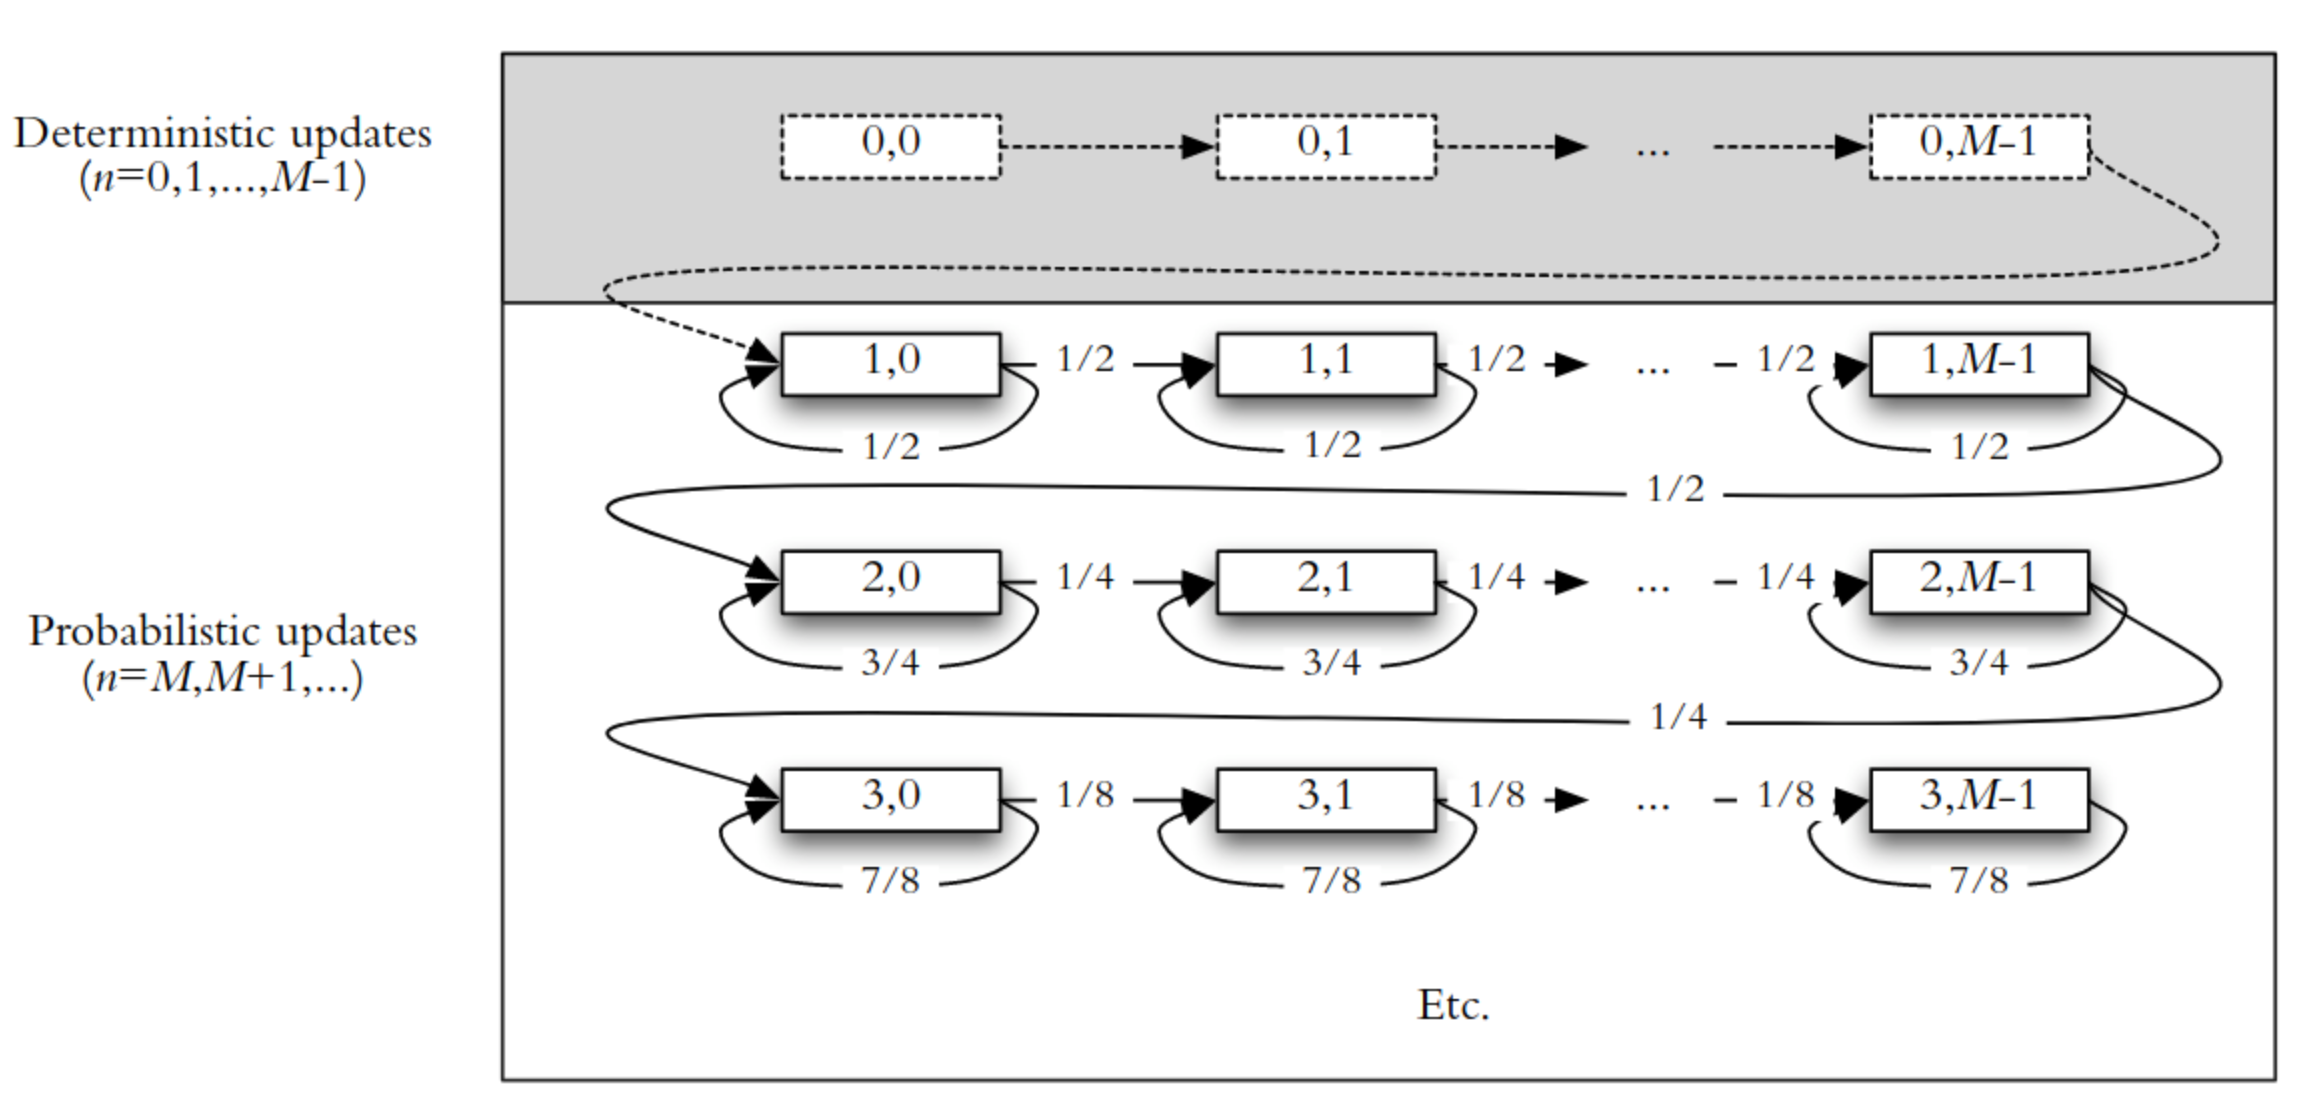
\includegraphics[width=0.9\linewidth]{figs/csuros.png}
    \caption{Csűrös' counter exemplified in graphical form.}
    \label{fig:csuros}
\end{figure}

\begin{algorithm}[ht!]
\caption{Csűrös' counter algorithm}
\label{alg:csuros}
\begin{algorithmic}
\Inputs{$book \gets$ string of text to be analysed

$d \gets$ design parameter}
\Initialize{$counter \gets$ data structure used for counting the occurrences of every word
            $RandomNumber \gets$ function that generates a number between 0 and 1
            \State $t \gets$ 0
            \State $u \gets$ 0}



\For{$word$ in $book$}
    \State $r_{number} = RandomNumber$
    \If{$r_{number}<(\frac{1}{2})^{t}$}

        \If{$word$ in $counter$}
            \State $counter[word]+=1$
            \State $u +=1$
        \Else
            \State $counter[word] \gets$ data structure
            \State $counter[word]=1$
            \State $u +=1$
        \EndIf for a specific number of occurrences $x$, with $p$ being the sampling probability:

    \EndIf
    \If{$u==2^d$}
        \State $t +=1$
        \State $u = 0$
    \EndIf
\EndFor
\end{algorithmic}
\end{algorithm}



For a specific number of occurrences $x$ with $p$ being the design parameter and $M = 2^p$, to calculate the expected count $f(x)$, it is used:

\begin{equation}
    x = (M +u)2^t-M
    \label{eq:csuros1}
\end{equation}
\begin{equation}
    f(x) = Mt + u
    \label{eq:csuros2}
\end{equation}

\noindent with $u$ and $t$ representing the variables in \autoref{alg:csuros}.

However, these equations are not enough because we have three unknown variables $f(x)$, $t$, and $u$, and only two different equations.
Nevertheless, it is known that $u$ is not larger than 8 and $t$ is the number of times $u$ hits the number 8.
Therefore, the following algorithm was developed:

\begin{algorithm}[ht!]
\caption{Csűrös' estimation algorithm}
\label{alg:csuros1}
\begin{algorithmic}
\Inputs{$x \gets$ specific number of occurrences

$d \gets$ design parameter}
\Initialize{$t \gets$ 0
            \State $u \gets$ 0
            \State $f(x) \gets$ 0}


 \While{$x>0$}
    
    \State $f(x) += (\frac{1}{2})^t$
    \State $u+=1$
    \State $x-=1$    

    \If{$u==2^d$}
        \State $t +=1$
        \State $u = 0$
    \EndIf

 \EndWhile


\end{algorithmic}
\end{algorithm}




